%!TEX root = ../thesis_phd.tex
%%%%%%%%%%%%%%%%%%%%%%%%%%%%%%%%%%%%%%%%%%%%%%%%%%%%%%%%%%%%%%%%%%%%%%%%%%%%%%%
% intro.tex: Introduction to the thesis
%%%%%%%%%%%%%%%%%%%%%%%%%%%%%%%%%%%%%%%%%%%%%%%%%%%%%%%%%%%%%%%%%%%%%%%%%%%%%%%%
\chapter{Introduction}
\label{intro_chapter}
%%%%%%%%%%%%%%%%%%%%%%%%%%%%%%%%%%%%%%%%%%%%%%%%%%%%%%%%%%%%%%%%%%%%%%%%%%%%%%%%

%\section{Overview}

Arguably the most mysterious particle of all is the neutrino.
This thesis aims to measure parameters which will remove some of that mystery.
Neutrinos are neutral particles of relatively small mass which are only
known to interact through the weak and gravitational forces, ignoring the
effects of the strong and electromagnetic forces.
Since they only couple to the subdominant forces, neutrino interactions are astonishingly rare; a neutrino traveling through a light year of lead has less than a 50\% chance of interacting.  From the perspective of particle physicists, the low probability of observing neutrino interactions has made their characterization an extremely elusive task.

Neutrinos undergo a curious phenomenon called oscillation, or the ability for members of the neutrino family to transform into other members.  The \nova experiment has built two detectors separated by a distance of nearly 1,000 km in order to observe neutrino oscillations.  This thesis aims to better measure the frequencies at which neutrino oscillate, particularly by improving the method by which neutrinos are identified within \nova detectors.

The data output from \nova detectors can be interpreted roughly as top and side view images of neutrino interactions.  In that sense, identification of neutrino interactions in \nova detectors can be seen as an image classification task.  The image classification community has made great strides through convolutional neural network classifiers.  Implementing that technique for interaction classification in \nova will be the central thrust of this thesis.


\section{The Standard Model}

High energy particle physics seeks to address age-old topic of describing the constituents of matter throughout the universe.  The Greek atomist theories are among the earliest attempts at answering this question.  Democritus is well known for putting forth the theory that all matter was made up of indivisible, or fundamental, particles called atoms.  Plato furthered this idea by proposing that the all matter was comprised of four basic elements: earth, air, fire and water \cite{berryman2008atomism}.  Dimitri Mendeleev made huge strides in understanding the structure of matter through the organization of the periodic table.  The elemental atoms represented in the periodic table, however, are not fundamental.  In similar manner, the Standard Model of particle physics represents our latest attempt to describe matter in terms of fundamental particles.  Of course, there is no guarantee that the particles of the Standard Model are truly fundamental, but no experiment has been performed to suggest otherwise.  A graphic which displays all of the particles in the Standard Model can be seen in figure \ref{sm}.


\begin{figure}[h]
  \begin{center}
    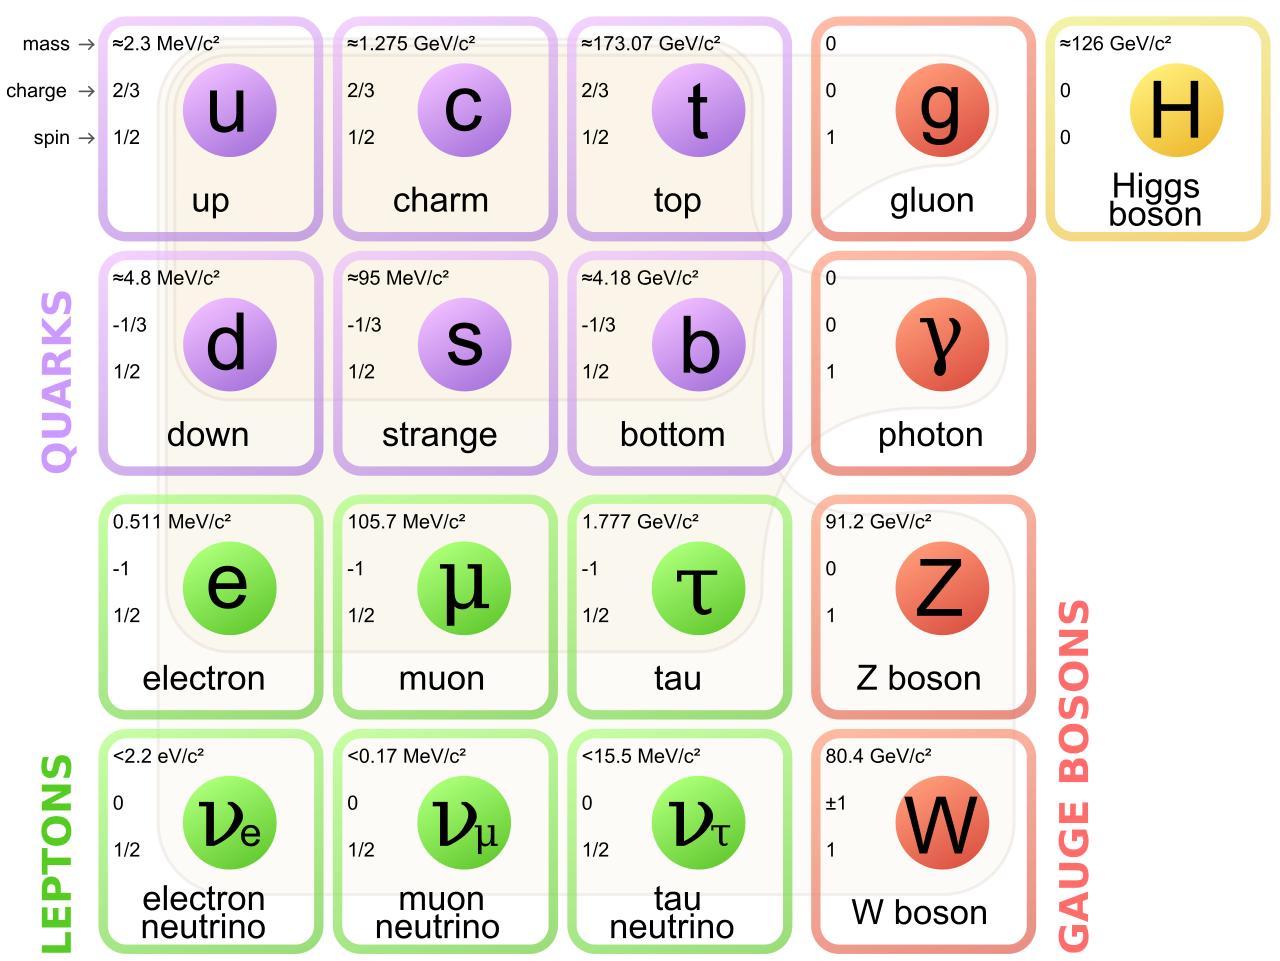
\includegraphics[width=0.6\textwidth]{figures/figures/sm.png}
  \end{center}
  \caption{Diagram which enumerates all of the fundamental particles in the standard model.}
  \label{sm}
\end{figure}

The standard model A particle is an entity with a distinct charge, mass, and spin.  Like charge and mass, spin the intrinsic property of a particle which represents its magnetic moment.  But spin also serves to distinguish fermions and bosons. Fermions have a half integer spin, e.g. $\frac{1}{2}, -\frac{1}{2}, \frac{3}{2}$, while bosons have integer spin.  Matter is primarily made up of the fermions in the Standard Model, all of which have a spin of $\pm \frac{1}{2}$.  The bosons in the Standard Model are force carriers, or in other words, they mediate the interactions of the electromagnetic, strong and weak forces.  All of the bosons in the standard model have a spin of $+1, 0, $ or $ -1$.  Each charged particle in the Standard Model is complimented by an antiparticle which has the same mass and spin, but opposite charge. \cite{halzen1984quarks}

Fermions are further grouped into two categories: quarks and leptons.  Atomic nuclei are built up from quarks; a proton is comprised up quarks and one down quarks, a neutron is comprised of two down quarks and one up quark.  Combinations of three quarks are known as baryons, while those of two quarks are called mesons.  Recent experiments have revealed particles which are likely to contain four or five quarks \cite{dias2013z_,barth2003evidence}.  Distinct baryons and mesons are not merely formed by different combinations of quarks, but also from excited states of those combinations.  Quarks in baryons and mesons are held together by the strong force, although they also interact through the weak and electromagnetic force.  Antiparticle compliments of quarks are known as antiquarks.  \cite{halzen1984quarks}

Leptons, on the other hand, do not interact through the strong force.  The most familiar example of a lepton is the electron, which make up the exterior region of atoms in matter.  The electron (e) has two heavier counterparts, the muon ($\mu$) and tau ($\tau$).  These three particles, along with their antiparticles, represent the charged leptons.  Each of the charge leptons can couple to a corresponding neutrino in weak interactions; thus the neutrinos are named after: electron neutrino (\nue), muon neutrino (\numu), and tau neutrino ($\nu_\tau$).

\section{History of Neutrino Physics}

\subsection{The Neutrino Hypothesis}

Mankind's first glimpse at the neutrino came in the early part of the 20th century along with studies of nuclear beta decay.  Discovered in 1896 by Henri Bequerel, beta decay was characterized by the mysterious ``beta rays" that were emitted by various types of radioactive material.  \cite{becquerelBeta}  By 1900, however, Becquerel had categorized beta rays as electrons, suggesting that beta decay involved a heavy atom emitting a relatively light, but fast moving electron.\footnote{
We now know beta decay to involve a neutron within a nucleus decaying into a proton, electron and electron antineutrino, as follows: 
\begin{equation*}      n \rightarrow p + e^- + \bar{\nu}_e  . \end{equation*}
Even though electrons were discovered in 1897 by J.J. Thompson in his examination of cathode rays \cite{thompson}, atomic structure was still shrouded in uncertainty.  Geiger, Mardsen and Rutherford's gold foil experiment found evidence of the nucleus 1909, but neutrons were not hypothesized until 1920 by Rutherford \cite{rutherfordNeutron} and remained undiscovered until work done in 1932 by James Chadwick. \cite{chadwickNeutron}
 } \cite{becquerelElec}  
James Chadwick measured the energy spectrum of beta decay electrons in 1914 and found that the spectrum was continuous rather than discrete and single-valued \cite {chadwickBeta}.  Chadwick's result was clearly inconsistent with the two-particle process that Becquerel presented; for a two-body decay, momentum conservation exactly predicts the momentum of each particle.  In the case of beta decay, emission of a relatively lightweight electron from a heavy atom should leave the atom stationary, specifically determining the energy of the electron .  Chadwick measured a range of electron energies much larger than the uncertainty in atomic recoil energy, clearly violating the two-particle model of beta decay.  

As a solution to this problem, in 1930 Wolfgang Pauli proposed that this decay could in fact be a three-body decay involving a third particle, which he then called a neutron, electrically neutral and also considerably lighter than a nucleus. \cite{pauliNeuProp}  Two years later the actual neutron we refer to today was discovered by Chadwick \cite{chadwickNeutron} and in 1934 Enrico Fermi proposed that Pauli's particle be called a ``neutrino." \cite{fermiNeuName} 

\subsection{Neutrino Discovery -- Methods and Observations}
\label{discovery}


Cowan and Reines made the first observation of neutrinos in 1956.  The neutrinos they observed were produced through beta decays in a nuclear reactor.  Since the field of particle physics had advanced considerably by this point, Cowan and Reines had enough information to expect the signal: 
\begin{equation} \label{beta} \bar{\nu}_e + p \rightarrow n + e^+.  \end{equation}
Detectors used in their experiment employed scintillation counters to register energy deposition from candidate events.  Neutrino events were selected by coincidence between a prompt electron-positron annihilation signal followed by a larger delayed neutron capture signal, shown in Figure~\ref{oscilloscope}.  The delay of the second signal spans the time for the fast-moving neutrons to thermalize, that is, to lose energy through nuclear scattering until reaching the energy scale required for capture. 
\begin{figure}[b!]
  \begin{center}
    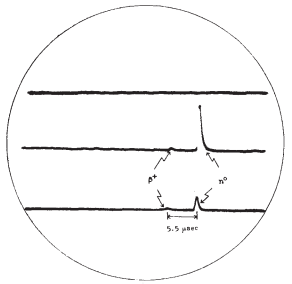
\includegraphics[width=0.6\textwidth]{figures/figures/cowanOscilloscope.png}
  \end{center}
  \caption{Oscilloscope trace from Cowan and Reines' experiment.  The small bump is the electron/positron annihilation signal, the large spike is the neutron capture signal.}
  \label{oscilloscope}
\end{figure}
Cowan and Reines measured a neutrino rate of 2.88 $\pm$ 0.22 counts/hour, representing a signal rate 3 times larger than the measured background.  \cite{cowan}  The neutrinos observed in this experiment were later classified as electron ``flavor''  neutrinos.

Neutrino physics grew in scope  with the discovery of a second class of neutrinos in 1962.  Lee and Yang made a prediction that there existed neutrinos associated with muons in addition to those associated with electrons.  They also made detailed calculations predicting cross sections for interaction \eqref{beta} as well as:
\begin{equation} \label{betaMinus} \nu_e + n^0 \rightarrow p^+ + e^- \end{equation}
\begin{equation} \label{betaMuMinus}\nu_\mu + n^0 \rightarrow  p^+ + \mu^- \end{equation}
\begin{equation} \label{betaMuPlus}\bar{\nu}_\mu + p^+ \rightarrow n^0 + \mu^+ . \end{equation}
The world's largest accelerator at the time was the Alternating Gradient Synchrotron (AGS) at Brookhaven National Lab.  AGS accelerated protons for collision upon a fixed target, resulting in production of charged pions.  The pions would then decay to yield muons and muon neutrinos as follows:  
\begin{equation} \label{pions} \begin{split}
\pi^+ \rightarrow \mu^+ + \nu_\mu {\ } \\
\pi^- \rightarrow \mu^- + \bar{\nu}_\mu.
\end{split} \end{equation}
An arrangement of lead and steel was placed in the beamline to absorb the muons.  Beyond the absorbers, spark chambers were deployed that would create sparks along the path traversed by charged particles.  Neutrinos, unaffected by the muon absorbers, interacted in the spark chambers according to \eqref{betaMuMinus} and \eqref{betaMuPlus} to produce muon ``tracks."  Activity in the spark chamber triggered a camera to produce photographs for analysis.  To eliminate cosmic ray background, events analyzed were required to pass a preselection by satisfying two criteria--- that the muon track must start and stop well within the spark chamber, and that their angle relative to the beam direction be less than $60^\circ$--- leaving behind 113 events over a background of 1800.  After surviving preselection, the remaining events were subdivided into four categories.  Of these events, 49 were labeled as ``short tracks," and eliminated as likely being caused by neutron background.  Another group of 22 were designated ``vertex events"  because they contained more than one track; not being representative of interactions \eqref{betaMuMinus} and \eqref{betaMuPlus}, these events were excluded.  Yet another 9 events were classified as ``showers" due to irregular track activity uncharacteristic of muons.  Thus, the final selection contained 34 candidate muon neutrino interactions with a single clean muon track \cite{numuDiscovery}.  In 1988, Leon Lederman, Melvin Schwartz, Jack Steinberger were awarded the Nobel Prize in Physics for the discovery of muon flavor neutrinos.

The force carriers for the weak force, the $W^\pm$ and $Z^0$ bosons, were discovered at the Super Proton Synchrotron (SPS) at CERN, thus opening up a new realm of inquiry for particle physics \cite{wBoson, zBoson}.  Along with the observation of these bosons came a measurement of their cross sections and decay rates.  $Z^0$ bosons are expected to decay to neutrinos and contribute to its decay rate, but these decays are typically unobservable in collider detectors; this deficit is typically called the invisible rate.  By measuring the total $Z^0$ decay rate as well as the rate observed through visible processes, the difference can be taken to obtain the invisible rate.  The measurement -- made using the ALEPH detector on the Large Electron Positron collider (LEP) at CERN -- determined of the total number of neutrino types that can interact via the weak force.  ALEPH determined the number of neutrino flavors to be consistent with three, ruling out the possibility of four neutrino flavors at the 98\% confidence level.  \cite{aleph}  Measurement of invisible $Z^0$ width, however, only dictates the number of neutrinos that interact weakly.  Neutrinos that do not interact weakly are known as sterile neutrinos.

The ALEPH measurement, on top of the previous associations of neutrinos with electrons and muons, suggested that the third neutrino type should be associated with taus.\footnote{Electrons ($e$), muons ($\mu$) and taus ($\tau$) are members of a class of fundamental particles known as leptons.  These three particles are the only leptons with electric charge; the remaining members of the lepton family are their associated neutrinos: \nue, \numu and $\nu_\tau$  }  An experiment called Direct Observation of Nu Tau (DONUT) was constructed at Fermilab to detect $\nu_\tau$ through interactions analogous with the electrons and muons:
\begin{equation} \label{tauCCMinus}\nu_\tau + n^0 \rightarrow  p^+ + \tau^- \end{equation}
\begin{equation} \label{tauCCPlus}\bar{\nu}_\tau + p^+ \rightarrow n^0 + \tau^+ . \end{equation}
Energetic protons taken from the Tevatron accelerator were directed into a tungsten beam dump to yield a shower of particles including heavy mesons.  The primary source of $\nu_\tau$ in the experiment was the $D_S$ meson through its decay:
\begin{equation}\label{nuTauDS}
D_S \rightarrow \tau + \nu_\tau
\end{equation}
Similar to the Brookhaven muon neutrino experiment, DONUT used an array of steel absorbers beyond the beam dump, but additionally implemented a set of deflecting magnets to steer muons and other light particles out of the beamline.  Downstream of the absorbers was a detector comprised of alternating layers two types of tracker modules: emulsion cloud chambers (ECC) and scintillating fiber trackers (SFT).  The ECC were assembled with sheets of photographic emulsion that would become exposed along the track of a fast moving charged particles.  This detection scheme provided precise spatial resolution for tracks required for identification of taus by a characteristic kink in their track 2 mm from the $\nu_\tau$ interaction point.  Interleaved between the ECC, the SFT was comprised of scintillating fibers that would produce light in the presence of charged particle radiation and transmit that light to image intensifiers for digitization.  The SFT was used to identify regions containing activity within the ECC for analysis.  In 2001 the DONUT collaboration published the results of this analysis; their paper reported the observation of four interactions compatible with \eqref{tauCCMinus} and \eqref{tauCCPlus} above an expected background of 0.34 events.  \cite{nuTau}

\subsection{The Solar Neutrino Problem}

In the 1960's Ray Davis and others set out to determine the flux of neutrinos incident upon the earth as a result of nuclear fusion within the sun.  Davis and his collaborators designed and built a detector based on a beta process  that converts chlorine atoms to argon atoms , namely: 
\begin{equation}\label{nuChlorCap}
{}^{37}Cl + \nu_e  \rightarrow {}^{37}Ar + e^-. 
\end{equation}
The cross section for this interaction was calculated in 1964 by John Bahcall \cite{bahcall}.  Davis' detector was a large tank (placed underground at the Homestake mine to reduce cosmic ray background) filled with an organic compound called perchloroethylene ($C_4Cl_8$).  \cite{davis}  Over time, the solar neutrino flux converted a measurable fraction of the chlorine atoms to argon.  Every few weeks, Davis would bubble helium through the tanks to collect the argon atoms and measure the amount collected.  Upon analysis, it was found that Davis' measured fluxes were a factor of three smaller than those predicted from solar models.  Many doubted Davis' measurement because it relied on radiochemical processes rather than event-by-event analysis; however, errors could not be found in the experiment.  Flux measurements were also made by the Kamiokande-II experiment and the Sudbury Neutrino Observatory (SNO) \cite{kamiokande, sno}.  All results were found to be consistent with Davis' measurements but inconsistent with the prediction.  The deficit in flux measured in these experiments became known as the ``solar neutrino problem."

The solution to the solar neutrino problem came in the form of neutrino oscillations, that is, the concept that neutrinos can change flavor as they propagate.  If neutrinos can change flavor, then some of the electron neutrinos produced in the sun would transform to muon and tau neutrinos before reaching earth.  As a result, the aforementioned experiments would indeed measure a diminished neutrino flux relative to the prediction.  

Bruno Pontecorvo first described neutrino oscillations in 1957 as a process that mixed neutrinos and antineutrinos  \cite{pontecorvo}.  These ideas were later expanded by Maki, Nakagawa and Sakata in 1962 to explain the small leptonic decay rate of hyperons\footnote{A hyperon is a particle comprised of one or more strange quarks, but no charm quarks or bottom quarks.} through the mixing of electron and muon neutrinos.  The theory of neutrino oscillations was later expanded to include tau neutrinos.  A detailed description of neutrino oscillations will come in the following section.

%%%%%%%%%%%%%%%%%%%%%%%%%%%%%%%%%%%%%%%%%%%%%%%%%%%%%%%%%%%%%%%%%%%%%%%%%%%%%%%%
